\documentclass{beamer}

\usepackage[french]{babel}
\usepackage[OT1]{fontenc}
\usepackage[utf8]{inputenc}

\definecolor{macouleur}{rgb}{.255,.243,.202}
\usecolortheme[named=macouleur]{structure}
\usetheme{AnnArbor}
\setbeamertemplate{blocks}[rounded, shadow=true]
\setbeamercolor{block title alert}{fg=white, bg=pink}

\title{Soutenance}
\subtitle{sujet : Développement en C d'une application de gestion de rendez-vous d'une clinique}
\institute[2017-2018]{Transmission des Données et Sécurité de l'Information}
\date{}
\author[L1TDSI]{Soutenu par : \\Cheikh Tidiane Thiam\\Thierno Mamoudou Sabaly}

\begin{document}

\begin{frame}[t]
\includegraphics[scale=0.45]{Logolacgaa.png}
	\titlepage
\end{frame}
\begin{frame}{Plan}
\textbf{Introduction}
\begin{enumerate}
\item Présentation du projet
\item Outils de développements
\item Système de sauvegarde
\item Architecture de l'application
\item Présentation de l'agenda
\end{enumerate}
\textbf{Conclusion}
\end{frame}
\begin{frame}{INTRDUCTION}
Enregistrer un rendez-vous dans un systeme informatique constitue le moyen le plus diligent et le plus efficient de nos jours, mais aussi le moyen le plus sûr pour les traitements et la sauvegarde de l'information. Pour concrétiser notre projet, nous spécifierons dans ces chapitres les outils de développements ainsi que les interfaces de l'application.
\end{frame}

\begin{frame}{Présentation du projet}
Le but de notre projet a été de rendre aisé la prise de rendez-vous dans une clinique. Celle-ci pourra en autant de simplicité enregistrer, modifier ou bien même décommander un rendez-vous. Après avoir fait critique de  l'existant et détecter certains anomalies en ce qui concerne les methodes dont les personnels d'une cliniques disposaient pour gérer les rendez-vous,une approche approche différente consiste à concevoir et à developper une application qui facilitera les insuffisances énumérés, feront l'objet de notre système baptisé agenda électronique.
Ce nouveau système disponible bientot vise à simplifier et à accelérer la prise de rendez-vous.
\end{frame}

\begin{frame}{Outils de Developpement}
Pour la mise en place d'une telle application, nous avons fait recours aux outils suivants : 
\begin{enumerate}
\item Le langage C, langage de programmation \pause
\item La SDL, bibliothèque graphique. \pause
\item SublimeText3, éditeur (IDE)
\end{enumerate}
\end{frame}

\begin{frame}{Système de sauvegarde}
\pause Pour la sauvegarde des données, nous travaillons avec les fichiers. \pause
Plus particulièrement, nous utilisons les fichiers`\textbf{ binaires}.
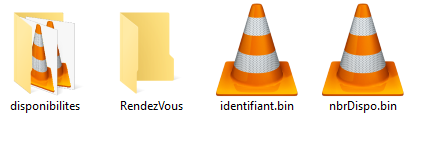
\includegraphics[scale = 0.5]{images/dansDmed.PNG}\\ \pause
Avec ces fichiers, nous sommes parvenu à construire notre propre base de données.
\end{frame}
\begin{frame}[t]{Architecture de l'apllication}
L'appliaction réalisée est complexe, mais simple et fiable. Nous étudions sa conception en deux étapes :
\begin{enumerate}
\item Préliminaires \pause
\item Mode de fonctionnement 
\end{enumerate}
\end{frame}

\begin{frame}{Préliminaires}
Avant toutes utilisation de l'application, il faudrait : \pause
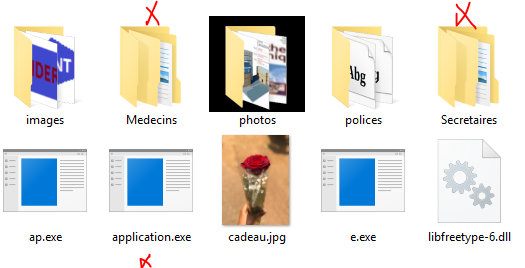
\includegraphics[scale = 0.45]{images/dossierInitiaux.PNG}\\
\end{frame}
\begin{frame}{Préliminaires}
Pour les médecins : \\ 

\includegraphics[scale = 0.65]{images/logodoct.jpg} 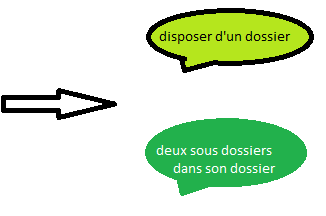
\includegraphics[scale = 0.65]{images/image1.PNG}\\ \pause
Le dossier porte le nom du médecin\\ \pause
Les sous-dossiers sont : \textbf{"disponibilites"} et \textbf{"RendezVous"}
\end{frame}
\begin{frame}{Préliminaires}
Et les secrétaires : \\

\includegraphics[scale = 0.45]{images/logosecretaire.jpg} 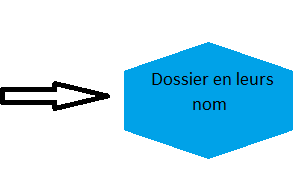
\includegraphics[scale = 0.45]{images/image2.PNG}

\end{frame}

\begin{frame}{Mode de fonctionnemnt}
Le fonctionnement de l'application est assuré par plusieurs fonctions communicante entre elles. Et voici les plus utiles : 
\end{frame}

\begin{frame}{Fonction de création de compte}
L'application est destinée aux secrétaires et aux médecins de la clinique.Elle impose à ses utilisateurs de disposer d'un compte.\\
c'est-à-dire : \\ \pause

\includegraphics[scale  = 0.5]{images/creationcompte.PNG} 
\includegraphics[scale = 0.5]{images/next.PNG}
\includegraphics[scale = 0.5]{images/CCsuite.PNG} 
\end{frame}

\begin{frame}{Fonction de connexion}
\pause
Impacte sur le dossier du médecin : \\ \pause

\includegraphics{images/con_impact.PNG}
\end{frame}

\begin{frame}{Fonction de création de disponibilité}
\pause Impacte sur le dossier du médecin : \\ \pause

\includegraphics[scale = 0.5]{images/dispo_imp.PNG}
\includegraphics[scale = 0.5]{images/next.PNG}
\includegraphics[scale = 0.5]{images/dispo_imp_suite.PNG}
\end{frame}

\begin{frame}{Fonction des création de rendez-vous}
\pause Impacte sur le dossier : \\ \pause
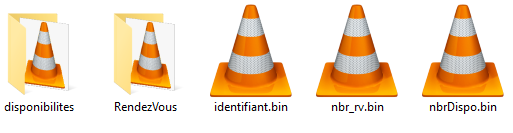
\includegraphics[scale = 0.5]{images/crv_impact}
\includegraphics[scale = 0.5]{images/next.PNG}
\includegraphics[scale = 0.5]{images/crv_impact_suite.PNG}
\end{frame}

\begin{frame}{Les autres fonctions}
\begin{enumerate}
\item Fonctions d'affichage \pause
\item Fonction permettant d'ordonner \pause
\item Fonction de suppression automatique \pause
\item...
\end{enumerate}
\end{frame}

\begin{frame}{Présentation de l'application}
Voyons un peu, dans cette partie l'apparence de l'application. Et s'en suivra une démonstration.
\end{frame}

\begin{frame}{Interface d'accueil}
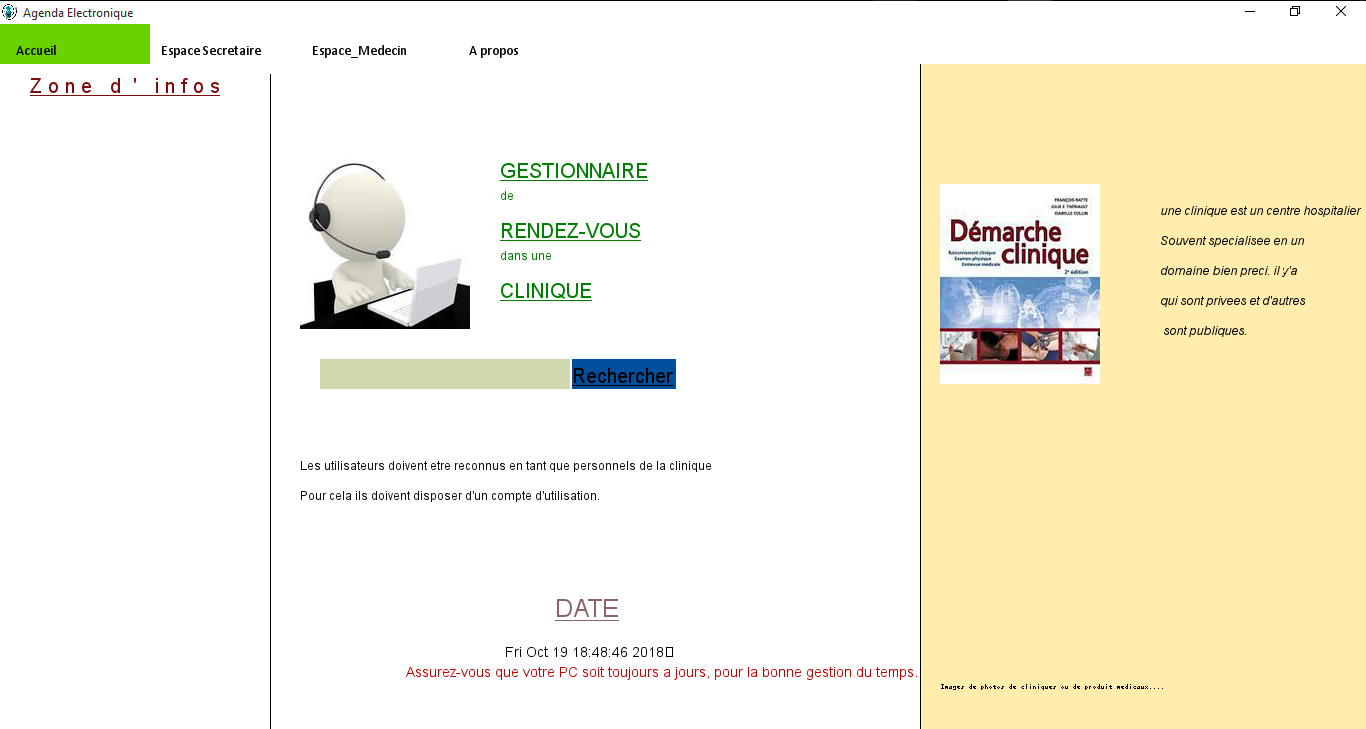
\includegraphics[scale = 0.35]{images/interf_acc.PNG}
\end{frame}

\begin{frame}{Interface d'accueille des secrétaires}
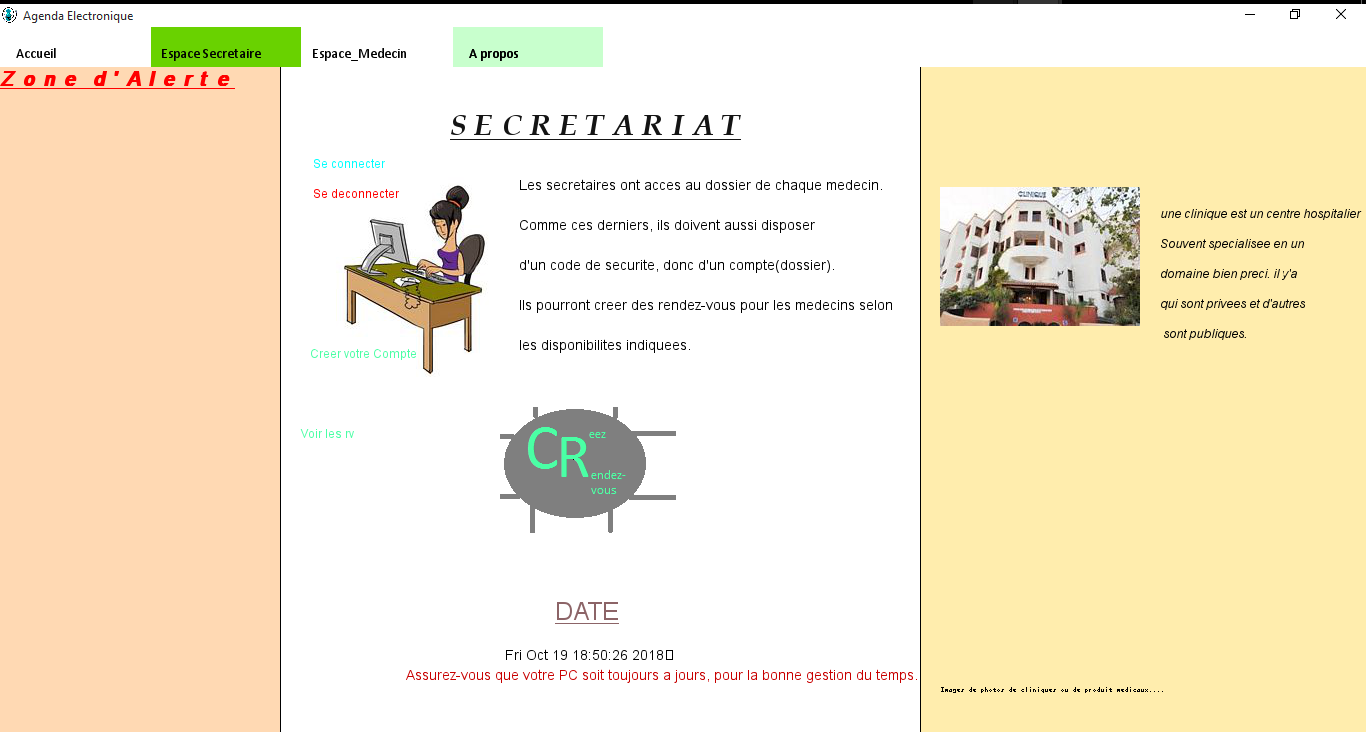
\includegraphics[scale = 0.35]{images/interf_acc_sec.PNG}

\end{frame}

\begin{frame}{Interface d'accueille des médecins}
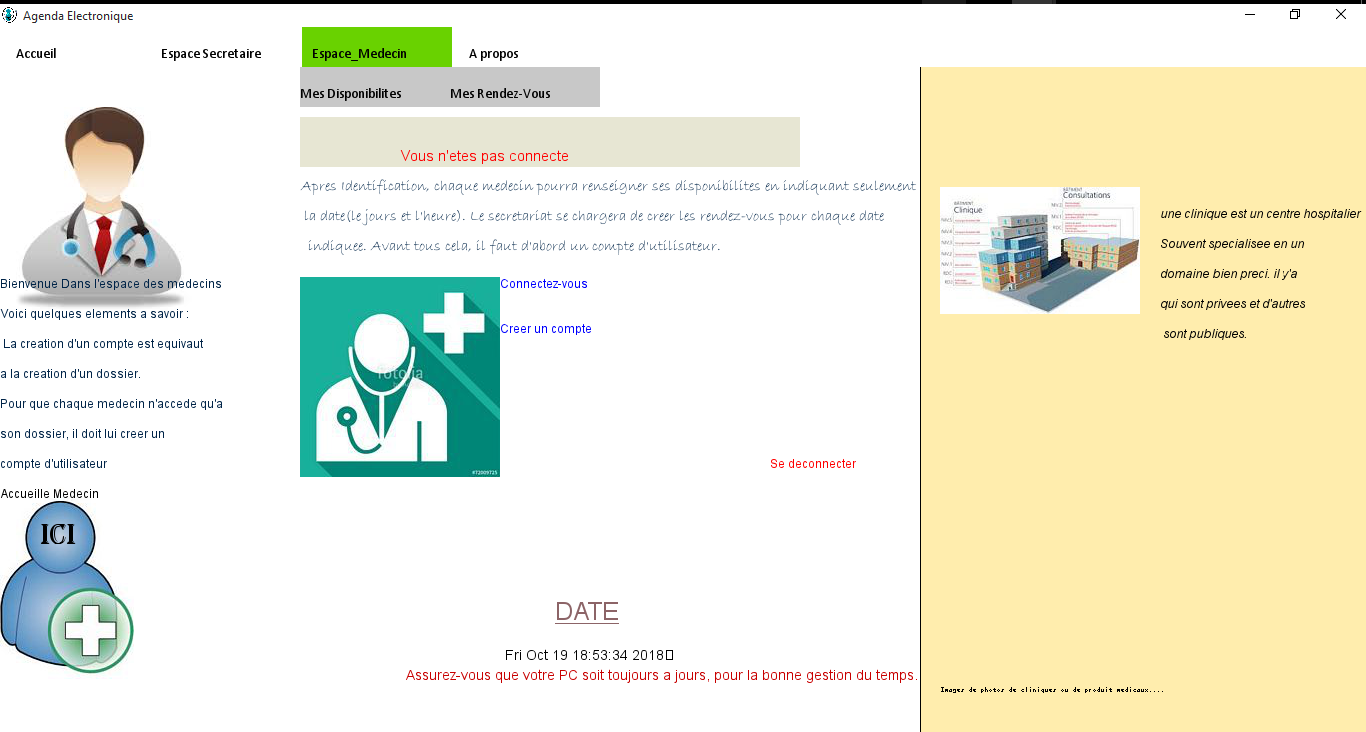
\includegraphics[scale = 0.35]{images/interf_acc_med.PNG}
\end{frame}

\begin{frame}{Interface des disponibilités}
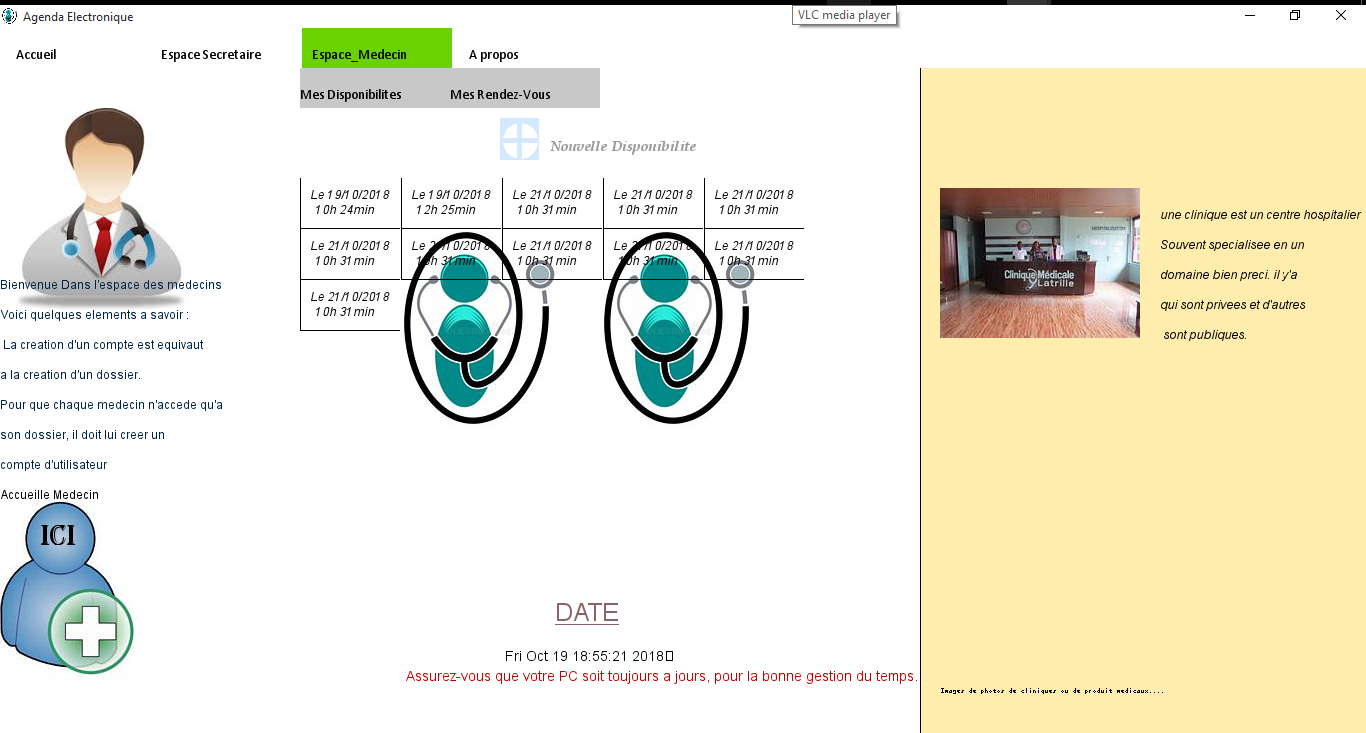
\includegraphics[scale = 0.35]{images/interf_dispo.PNG}
\end{frame}

\begin{frame}{Interface des rendez-vous}
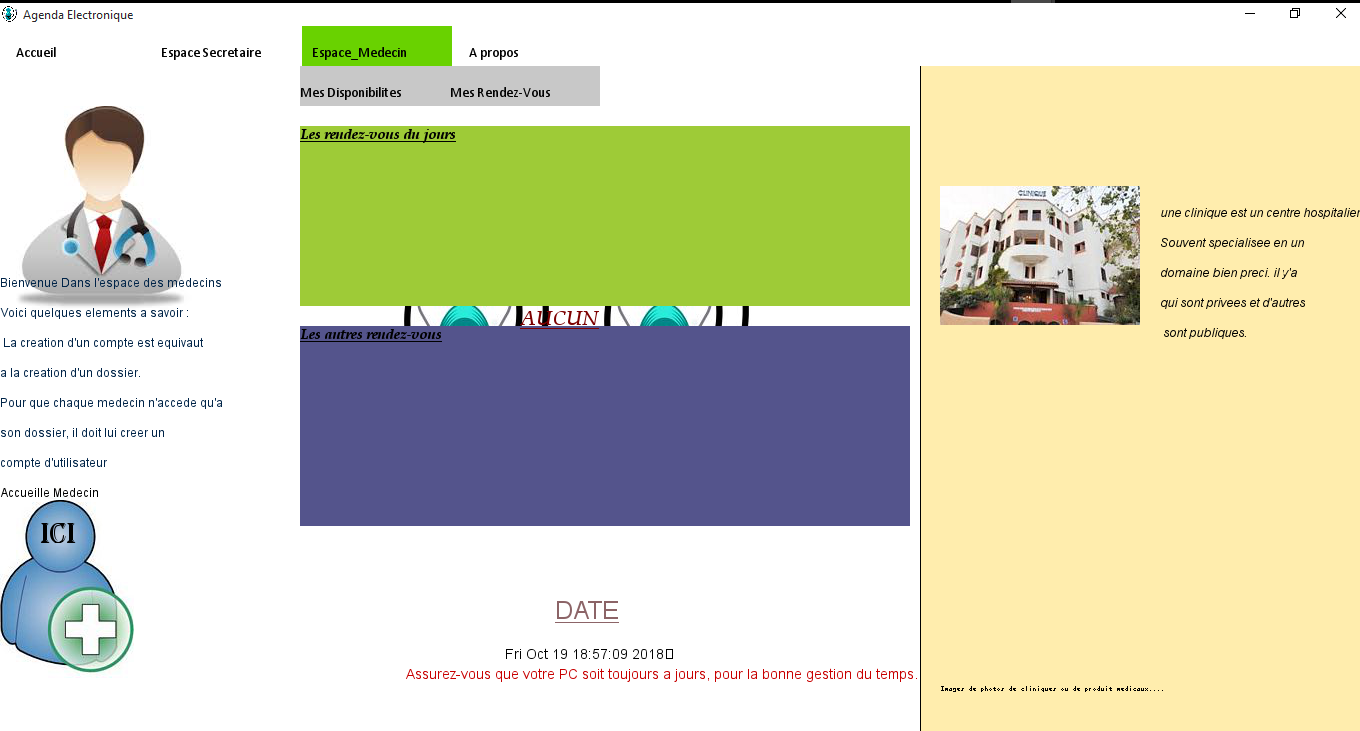
\includegraphics[scale = 0.35]{images/interf_rv.PNG}
\end{frame}

\begin{frame}{Interface pour créer un rendez-vous}
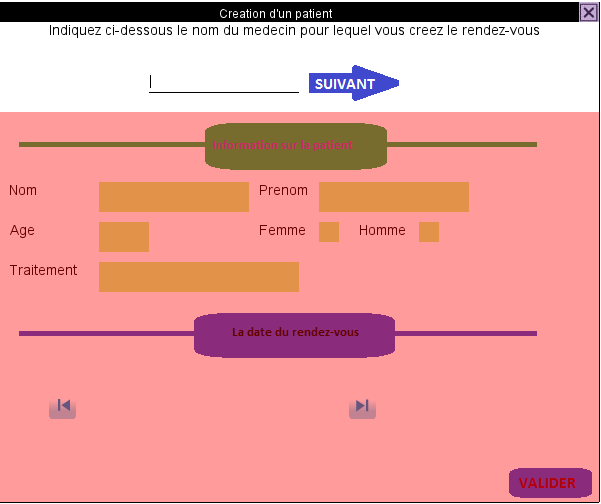
\includegraphics[scale = 0.45]{images/interf_crv.PNG}
\end{frame}

\begin{frame}{Démonstration}
\end{frame}

\begin{frame}{Conclusion}
Nous avons présenté au cours de ce travail, les différentes étapes de la conception et la réalisation de notre agenda électronique.
\\Afin de satisfaire les besoins des utilisateurs, nous avons commencé par nous poser des questions concernant la gestion des rendez-vous dans une clinique, ainsi nos réponses et certains critiques externes nous ont beaucoups aidés à atteindre nos objectifs et surtout de savoir les fonctionnalités à considérer durant le développement de l'agenda électronique.
Ce projet a fait l'objet d'une expérience intéressante, qui nous a permis de pousser nos connaissances dans le domaine de la programmation. Nous espérons que cette solution répondra aux attentes de tout utilisateur au sein d'une clinique.
\end{frame}
\end{document}